\documentclass[12pt]{article}
\usepackage{sbc-template}
\usepackage{graphicx,xurl,placeins}
\graphicspath{{figures/lab02/}{paper/figures/lab02/}}
\usepackage[utf8]{inputenc}
\usepackage[T1]{fontenc}
\usepackage[brazil]{babel}
\usepackage{amsmath,amssymb,booktabs}
\usepackage[hidelinks]{hyperref}
\sloppy
\title{Além do Beta Tradicional: Suplemento de Métodos e Validação}
\author{Robson Dias Ferreira\inst{1}}
\address{Instituto de Informática -- Universidade Federal do Rio Grande do Sul (UFRGS)\\
Programa de Pós-Graduação em Computação (PPGC)\\
Disciplina CMP609 -- Introdução aos Métodos Computacionais em Finanças
\email{}}
\begin{document}
\maketitle
Material complementar ao artigo. Mantém os experimentos individuais
anteriores e a previsão exploratória com seus alvos e limitações próprios.
Os resultados agregados posteriores não recebem a garantia do envelope.
\section{Calibração individual e complemento Monte Carlo}
Os experimentos de desenho fixo seguem a organização de objetivos,
mecanismos, estimandos e desempenho de Morris et al. \cite{morris2019}.
Preservam mercado, calendários, máscaras,117 caminhos únicos e janelas
sobrepostas, com 1.000 réplicas independentes por mecanismo.
No gerador $y_{it}=\beta_{0i}m_t+\delta_iD_tm_t+\sigma_i h_tu_{it}$,
$\beta_{0i}$ e $\sigma_i $ são calibrados uma vez por ativo; não são
parâmetros financeiros conhecidos. As inovações combinam componentes
comum e individual com pesos $\sqrt{0,3}$ e $\sqrt{0,7}$.

A classe protegida do complemento contém três mecanismos declarados:
normal iid, componentes t5 padronizados com escala heterocedástica
dependente do mercado defasado, e essa construção com AR(0,3).
Misturar componentes t5 não torna sua soma exatamente t5.
Adicionam-se, fora dessa classe, estresses GARCH t5
($\omega=0,03$, $\alpha=0,05$, $\beta=0,92$), quebra de escala
em 2020 e AR(0,6) \cite{bollerslev1986}. Fórmulas, inicializações,
sementes e grades completas são preservadas nos protocolos.

O estatístico complementar usa resíduos divididos por $1-h_{it}$,
com $h_{it}$ a alavancagem OLS, no sandwich Bartlett 5
\cite{mackinnonwhite1985}. Esse híbrido HC3--HAC5 não possui
validade finita automática. Os ensaios com HC3/Holm e maxT também
não corrigiram uniformemente a calibração; seus resultados e relações
com bootstrap dependente/máximos gaussianos
\cite{shao2010,chernozhukov2013} permanecem no registro técnico.

Para cada desenho equivalente $d $ e mecanismo $g $, o banco independente final contém
$B=99.999$ estatísticos $T=\widehat\Delta/\widehat{se}_{HC3-HAC5}$
sob a nula, em três fluxos de 33.333. Define-se
\begin{equation}
p_{dg}(T_i)=\frac{1+\sum_{b=1}^{B}\mathbf{1}(|T_{dgb}|\ge|T_i|)}{B+1},
\quad p_{i,env}=\max_{g\in\{1,2,3\}}p_{d(i)g}(T_i).
\end{equation}
Postos assinados unilaterais atendem aos testes anuais e postos
bilaterais ao contraste temporal \cite{dufour2006,phipson2010}.
O mapa $d(i)$ preserva datas, máscara e tipo de contraste. O catálogo
contém 25 desenhos: sete estáticos, 14 anuais e quatro entre metades.
Um banco é reutilizado somente quando essas características coincidem;
não se mistura a distribuição de máscaras diferentes.

Se $C\gamma=0$ é a nula do contraste no desenho $X_d $ e
$y=X_d\gamma+\sigma u $, então
$C\widehat\gamma(y)=\sigma C\widehat\gamma(u)$ e
$\widehat{se}(y)=\sigma\widehat{se}(u)$ para $\sigma>0$:
o resíduo OLS elimina $X_d\gamma $, enquanto alavancagens e pesos
dependem apenas do desenho. Isso justifica a invariância usada no banco.
O perfil temporal de escala e o coeficiente AR continuam fixados pelo
mecanismo; não são parâmetros desconhecidos que se cancelam livremente.
Sob um desses mecanismos e com banco independente, a permutabilidade entre
banco e estatístico nulo produz valor-p superuniforme; tomar o máximo
protege a união finita e Holm permite dependência entre ativos.
Essa garantia considera banco e estatístico conjuntamente, não
cada banco fixado; não abrange qualquer lei financeira ou erro na
construção dos retornos. Os estresses adicionais não ampliam a garantia.

Reportam-se cobertura, erro familiar (FWER), potência e incerteza
Monte Carlo. Wilson 95\% acompanha frequências familiares; com 1.000
réplicas, o maior erro padrão binomial é 1,581 ponto percentual.
O piso de valor-p final é $10^{-5}$; intervalos binomiais de cauda
são pontuais e não ICs da decisão ajustada. Preservam-se o banco
anterior de 9.999 e o primário HAC5, sem extensão seletiva da cauda
ou escolha de método pelo número de rejeições. A grade de efeitos
conhecidos não define margem de equivalência ou poder observado
retrospectivo.

\section{Resultados da calibração individual}
\label{sec:calibracao}
A calibração inicial HAC5 mostra subcobertura: na década,93,595\%
sob erros normais,93,429\% sob componentes t5 heterocedásticos e
91,841\% com AR0,3. As FWERs estáticas sob nulidade global são
7,9/6,7/5,9\%, com Wilson 95\% de[6,38;9,74], [5,31;8,42]
e[4,60;7,54]\%. Holm depende de valores-p individuais válidos:
o ajuste não corrige sua descalibração. Ensaios intermediários HC3
e maxT também apresentam falhas, preservadas no registro técnico.

O envelope final reduz essas frequências nos mecanismos declarados
(Tabela~\ref{tab:mc-e}), mas a avaliação sob nulidade global não
certifica toda configuração de nulas e alternativas. Diagnósticos
anteriores de IUT no limite produziram FWER HAC5 de 2,6 a 47,4\%,
contra zero a 0,6\% para o envelope; são amplitudes entre cenários,
não ICs nem prova geral de controle forte. Alguns limites Wilson
da tabela ultrapassam 5\%; os três últimos estresses permanecem
fora da classe protegida.

\begin{table}[htbp]
\centering
\caption{FWER do envelope final sob nulidade global(\%). Mil réplicas
por mecanismo; banco independente de 99.999 por mecanismo protegido.
Colchetes: Wilson 95\% Monte Carlo. Os três últimos são estresses
fora da classe protegida.}
\label{tab:mc-e}
\begin{tabular}{lcc}
\toprule
Mecanismo & Estática (197) & Temporal (474) \\
\midrule
Normal iid & 4,3 [3,21;5,74] & 0,4 [0,16;1,02] \\
t5 heteroscedástica & 3,3 [2,36;4,60] & 0,9 [0,47;1,70] \\
t5 heteroscedástica AR0,3 & 3,8 [2,78;5,17] & 1,5 [0,91;2,46] \\
t5 GARCH & 4,3 [3,21;5,74] & 0,5 [0,21;1,17] \\
t5 quebra de variância & 2,3 [1,54;3,43] & 0,6 [0,28;1,30] \\
t5 heteroscedástica AR0,6 & 4,9 [3,73;6,42] & 1,9 [1,22;2,95] \\
\bottomrule
\end{tabular}

\end{table}

Nas observações reais, VULC3 década mantém $p_{env}=0,00010$
e $p_{Holm197}=0,01970$, com nove excedências no mecanismo
dominante; não está no piso do banco final. Os três fluxos dão
valores ajustados 0,01182/0,02955/0,02955. BBDC4 apresenta
0,09408 no conjunto e 0,09996/0,08820/0,10584 nos fluxos.
A concordância das decisões reduz a preocupação com resolução
Monte Carlo, sem replicação empírica independente. O intervalo
binomial pontual da cauda dominante de VULC3 é aproximadamente
[0,000041;0,000171]; não é intervalo da decisão de Holm.

\section{Extensão exploratória de previsão do retorno seguinte}
\label{app:previsao}
Este exercício é preservado para transparência, mas tem alvo distinto
da assimetria e da previsão de exposição futura. Não constitui evidência
para as hipóteses centrais.

\subsection{Desenho e alvo da calibração}
Prevê-se o log-retorno do ativo na próxima sessão. A avaliação com
origens móveis \cite{hyndman2021} usa 252 sessões passadas e atualização
mensal;504 é sensibilidade. Comparam-se zero, média histórica,
regressão tradicional e condicional. As regressões usam os mesmos
pares, excluem mercado zero na estimação e mantêm os pisos 200/60/95\%
e de variância. Se houver insuficiência, ambas recuam à média passada.

Um AR(1) de mercado é ajustado apenas na janela de treino. Com
$\mu_t=\widehat a_m+\widehat\rho m_{t-1}$, inovações centradas
passadas $\widehat\epsilon_b $ e retas condicionais $g_i(x)$,
\begin{equation}
\widehat r^{cond}_{it}=\frac{1}{W-1}\sum_{b=1}^{W-1}
 g_i(\mu_t+\widehat\epsilon_b).
\end{equation}
A reta tradicional é integrada sobre as mesmas inovações; no ponto
exatamente zero usa-se seu intercepto. O sinal de $m_t $ realizado
nunca entra na previsão; serve apenas à decomposição posterior da perda.
Os 80 ativos são avaliados em 2019--2025, e os 117 em 2024--2025.
Os 80 comuns reutilizam as previsões recentes: o intervalo preditivo
comum 2024--2025 difere do comum descritivo 2021--2025.

Oito configurações preservam janelas, variantes de caixa/eventos,
máscara do quarto trimestre de 2024 da Light e proteção causal de lacunas já conhecidas em cada
origem. Exportam-se MSE, MAE,$R^2_{OS}$ contra zero/média e diferença
de perdas tradicional menos condicional. ICs de ganho utilizam 1.999
reamostragens síncronas das perdas, blocos 21/42/63, sem reestimar
modelos dentro de cada sorteio. A escolha retrospectiva dos ativos,
dados revisados e inspeção prévia dos anos impedem chamar o exercício
de holdout prospectivo intocado.

A calibração usa o ganho esperado
\begin{equation}
G_i^*=E\!\left[\frac{1}{n_i}\sum_{t\in\mathcal V_i}
 \{(y_{it}-\widehat f^T_{it})^2-(y_{it}-\widehat f^C_{it})^2\}
 \mid m_{1:T},\mathcal V_i,\mathcal M\right],
\end{equation}
condicional a todo o mercado observado, máscaras e lei geradora
especificada. Operadores lineares reestimam os modelos dos ativos
em cada réplica usando o passado. Com $q^j_{it}$ selecionando retorno
alvo menos os pesos da previsão $j $, o risco exato é
$(q^j_{it}\mu_i)^2+q^j_{it}\Sigma_i(q^j_{it})'$, incluindo
covariância treino--alvo sob AR. O mercado realizado entra na avaliação
desse oráculo, não no previsor. Não se calibra incerteza conjunta de
mercados futuros ou dos parâmetros geradores.

Simulam-se seis cenários (erros normais iid/GARCH/AR0,3,
$\delta=0/0,25$),1.000 réplicas cada, em 394 casos: duas janelas
vezes 80+117 ativos. Os 80 comuns não acrescentam casos.
ICs marginais são comparados a intervalos por máximo dos desvios
bootstrap absolutos padronizados pelo desvio-padrão bootstrap de cada
ativo. Esse denominador fica fixo nos sorteios; o quantil 0,9875
em cada um dos quatro grupos implementa Bonferroni entre grupos.
A avaliação é condicional aos bancos de reamostragem fixos e mede
cobertura, sem presumi-la pelo nome do procedimento.

\subsection{Resultados e cobertura}
O ganho relativo mediano de MSE muda de sinal entre recortes
(Tabela~\ref{tab:previsao}). Na configuração primária,43/80 ativos
longos,39/80 comuns e 55/117 recentes têm redução de MSE.
As medianas de $R^2_{OS}$ contra zero são negativas nos três recortes.
Uma melhora frente a outra regressão pode coexistir com desempenho
inferior ao referencial zero; contagens não demonstram superioridade
populacional ou econômica.

\begin{table}[htbp]
\centering
\caption{Previsão N252: medianas entre ativos. Ganho relativo
$100(1-MSE_{cond}/MSE_{trad})$;$R^2_{OS}$ contra zero.
Os 80 comuns reutilizam previsões dos 117.}
\label{tab:previsao}
\begin{tabular}{lrrr}
\toprule
Recorte & Ativos & Ganho MSE (\%) & $R^2_{OS}$ vs zero (\%)\\
\midrule
80, 2019--2025 & 80 & 0,00527 & -0,9672\\
80 comuns, 2024--2025 & 80 & -0,00033 & -0,4930\\
117, 2024--2025 & 117 & -0,00089 & -0,4834\\
\bottomrule
\end{tabular}

\end{table}
\begin{figure}[!htbp]
\centering
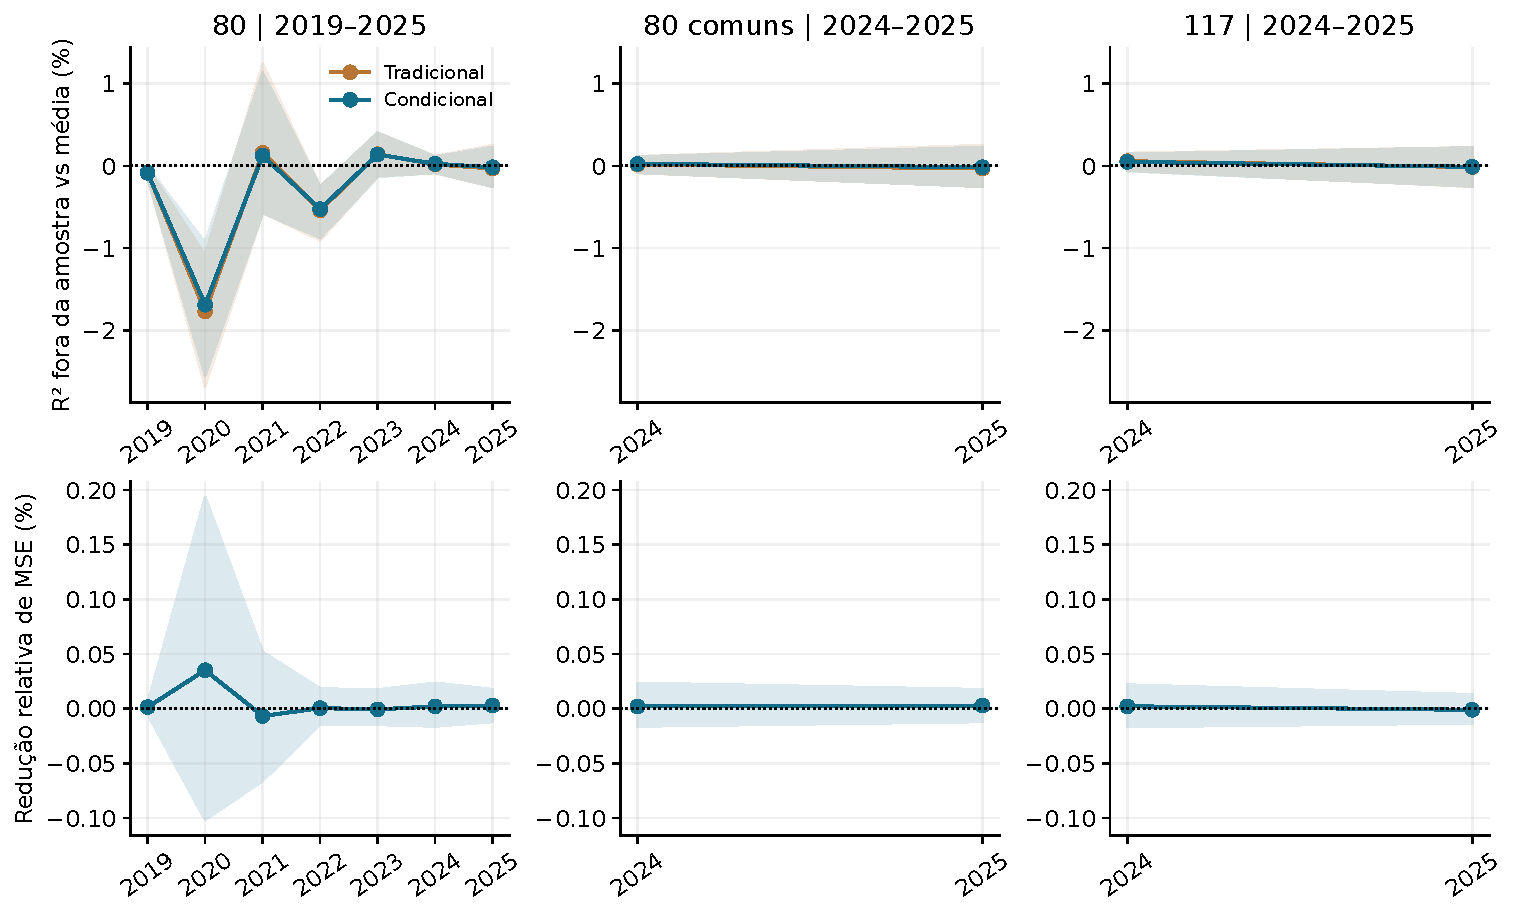
\includegraphics[width=\textwidth]{lab03d_previsao_anual.pdf}
\caption{Previsão histórica com cortes temporais estritos. Medianas/IQR
entre ativos por ano. Linha zero: igualdade de MSE ao referencial;
segunda linha: redução de MSE condicional ante o tradicional.}
\label{fig:previsao}
\end{figure}

Com 504 sessões, os ganhos medianos são aproximadamente
0,01573/0,000064/0,000021\%, mantendo diferenças pequenas.
Essa sensibilidade não substitui a janela 252 após observar resultados.
Não foram avaliados custos, alocação ou retorno de uma estratégia.

A calibração contra $G_i^*$ expõe cobertura marginal média de 88,51
a 93,06\%, abaixo de 95\%. A cobertura conjunta dos 394 é zero
nas 1.000 réplicas de cada cenário/bloco; esses ICs marginais não
foram construídos para cobertura conjunta. Sob $\delta=0$, usá-los
para declarar ao menos um ganho positivo produz FWER99,7--100\%.

Os intervalos por máximo elevam a cobertura conjunta, mas esta varia
de 98,4--99,2\% em blocos 21,94,8--97,0\% em 42 e 87,4--90,4\%
em 63 (Figura~\ref{fig:previsao-e}). Sob GARCH,$\delta=0,25$
e bloco 63, é 87,6\%, Wilson 95\%[85,41;89,50]. Não se escolhe
bloco 21 porque teve resultado favorável. Nenhum limite conjunto
inferior observado é positivo em qualquer janela/bloco; sob
$\delta=0,25$, a potência média para ganhos verdadeiros é inferior
a 0,04\%. Logo, os intervalos continuam exploratórios e a ausência
de rejeição não estabelece igualdade preditiva.

\begin{figure}[!htbp]
\centering
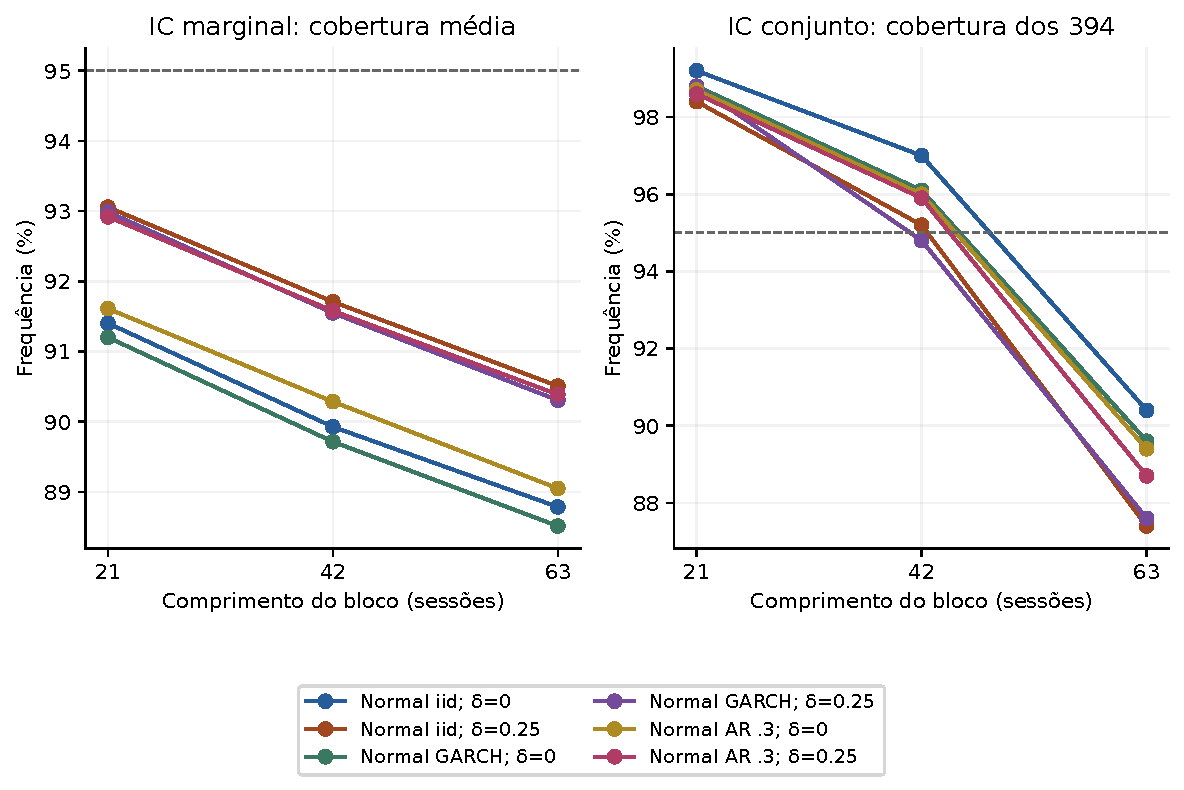
\includegraphics[width=\textwidth]{lab03e_cobertura_previsao.pdf}
\caption{Cobertura nos seis cenários preditivos,1.000 réplicas cada.
Marginal: média entre ativos; conjunta: cobertura dos 394 casos pelo
intervalo por máximo. Tracejado:95\%. Condicional ao mercado observado.}
\label{fig:previsao-e}
\end{figure}
\FloatBarrier


\section{Calibração agregada e sensibilidades completas}
\begin{table}[htbp]\centering\small
\caption{Calibração agregada sob nulidade global. FWER ajustada e
Wilson95\% Monte Carlo;1.000 réplicas por mecanismo, bloco21.}
\begin{tabular}{lrrrr}
\toprule
Mecanismo & FWER10 (\%) & Wilson95\% & FWER4 (\%) & Wilson95\%\\
\midrule
Normal iid & 1,6 & [0,99;2,58] & 2,1 & [1,38;3,19]\\
t5 heteroc. & 2,0 & [1,30;3,07] & 3,2 & [2,28;4,48]\\
t5 AR0,3 & 2,0 & [1,30;3,07] & 4,0 & [2,95;5,40]\\
GARCH t5 & 2,0 & [1,30;3,07] & 1,8 & [1,14;2,83]\\
Quebra t5 & 3,1 & [2,19;4,37] & 3,9 & [2,87;5,29]\\
t5 AR0,6 & 2,8 & [1,94;4,02] & 5,6 & [4,34;7,20]\\
\bottomrule
\end{tabular}

\end{table}
\begin{figure}[htbp]\centering
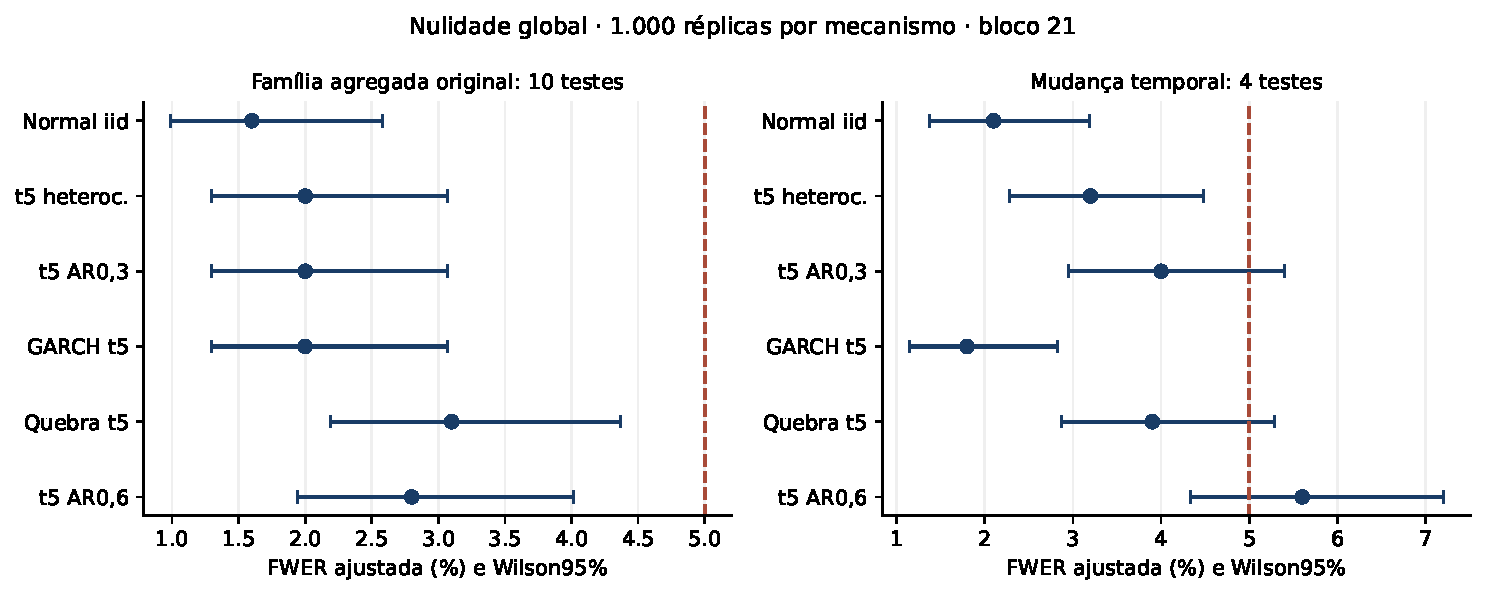
\includegraphics[width=\textwidth]{lab03g_calibracao.pdf}
\caption{Erro familiar sob nulidade global. Wilson 95\% é incerteza
Monte Carlo. Bancos, mercado e parâmetros geradores são fixados;
os três últimos mecanismos são estresses.}
\end{figure}
As 84.000 linhas de replicações, 252 taxas por caso e 24 taxas familiares
estão nos exports públicos. Incluem cobertura marginal, rejeição bruta
e ajustada, viés, erro-padrão e intervalos Monte Carlo. Não abrangem
mercados futuros, outros comprimentos ou os modelos dinâmicos/semanais.
As 66 linhas observadas e seus sorteios preservam todos os blocos,
estimativas, intervalos, status e valores-p; não se omitem sensibilidades.
\begingroup\small\bibliographystyle{sbc}\bibliography{references_artigo}\endgroup
\end{document}
